\documentclass[12pt,a4paper]{article}

% --- Настройка языка и шрифтов для LuaLaTeX ---
\usepackage{fontspec}
\defaultfontfeatures{Ligatures=TeX,Scale=MatchLowercase}

\setmainfont{Alice-Regular}[
    Path=font/,
    Extension=.ttf,
    BoldFont = Alice-Regular,
    ItalicFont = Alice-Regular,
    BoldItalicFont = Alice-Regular,
    BoldFeatures = {FakeBold=1.6},
    ItalicFeatures = {FakeSlant=0.2},
    BoldItalicFeatures = {FakeBold=1.6,FakeSlant=0.2}
]

\newfontfamily\cyrillicfont{Alice-Regular}[
    Path=font/,
    Extension=.ttf,
    BoldFont = Alice-Regular,
    ItalicFont = Alice-Regular,
    BoldItalicFont = Alice-Regular,
    BoldFeatures = {FakeBold=1.6},
    ItalicFeatures = {FakeSlant=0.2},
    BoldItalicFeatures = {FakeBold=1.6,FakeSlant=0.2}
]

\usepackage{polyglossia}
\setmainlanguage{russian}
\setsansfont{TeX Gyre Heros}
\setmonofont{TeX Gyre Cursor}

\usepackage{graphicx}        					% Графика
\usepackage{amsmath, amsfonts, amssymb, amsthm}	% Математика
\usepackage{mathtools}
\usepackage{chemfig}
\usepackage[version=4,arrows=pgf-filled,
textfontname=sffamily,
mathfontname=mathsf]{mhchem}
\usepackage[protrusion=false]{microtype}       % Микротипографика
\usepackage{braket} 						% Braket нотация для квантовой механики
\usepackage{unicode-math} 					% Современный пакет для математики в LuaLaTeX
\usepackage{longtable}       				% Таблицы с разрывом страниц
\usepackage{tikz}           				% Рисование
\usepackage[europeanresistors]{circuitikz}	% Рисование электрических схем в европейском стиле
\usepackage{listings}						% Для отображения кода
\usepackage{tabularx}       				% Для таблиц во всю ширину
\usepackage{array}		  					% Для расширенных возможностей таблиц
\usepackage{float}          				% Для точного позиционирования фигур
\usepackage{pgfplots}                          % Для построения графиков
\usepackage{caption}                           % Для настройки подписей к рисункам и таблицам
\usepackage{xfp}                               % Для вычислений в LaTeX
\usepackage{luacode}                           % Для выполнения Lua-кода в документе    
\pgfplotsset{compat=1.18}
\usepackage[paper=letterpaper,
            top=20mm,
            bottom=20mm,
            left=10mm,
            right=10mm,
            footskip=0.4in
]{geometry}

\usetikzlibrary{arrows.meta}

% --- Колонтитулы ---
\usepackage{fancyhdr}
\pagestyle{fancy}
\fancyhf{}

% --- Теоремы и окружения ---
\theoremstyle{plain}
\newtheorem{theorem}{Theorem}[section]
\newtheorem{lemma}[theorem]{Lemma}
\newtheorem{proposition}[theorem]{Proposition}
\newtheorem{corollary}[theorem]{Corollary}

\theoremstyle{definition}
\newtheorem{definition}[theorem]{Definition}

\theoremstyle{remark}
\newtheorem{remark}[theorem]{Remark}

\numberwithin{equation}{section}


\renewcommand{\headrulewidth}{0.4pt}
\renewcommand{\footrulewidth}{0.4pt}
\renewcommand\lstlistingname{Исходный код}

\lstdefinestyle{main}{
	backgroundcolor=\color{gray!8},   
	commentstyle=\color{green!50!black},
	keywordstyle=\color{blue!80!black},
	numberstyle=\small\color{darkgray},
	stringstyle=\rmfamily\color{orange!90!black},
	basicstyle=\ttfamily\small,
	breakatwhitespace=false,         
	breaklines=true,                   
	keepspaces=true,                 
	numbers=left,                    
	numbersep=8pt,                  
	showspaces=false,                
	showstringspaces=false,
	showtabs=false,                  
	tabsize=4
}	

\lstset{style=main}

% --- Настройка подсветки синтаксиса для MOPAC / WinMOPAC ---
\lstdefinelanguage{MOPAC}{
	alsoletter={.-},
	otherkeywords={=},
	keywords={AM1, PM3, RM1, MNDO, RHF, UHF, BFGS, EF, BONDS, GEO-OK, VECTORS, DENSITY},
	keywords=[2]{GNORM, CHARGE},
	keywords=[3]{=},
	keywords=[4]{0, 0.1, 1},
	sensitive=false
}

\lstdefinestyle{mopac}{
	language=MOPAC,
	backgroundcolor=\color{gray!10},
	basicstyle=\ttfamily\small,
	keywordstyle=\color{blue!80!black}\bfseries,
	keywordstyle=[2]\color{teal!80!black}\bfseries,
	keywordstyle=[3]\color{orange!80!black}\bfseries,
	keywordstyle=[4]\color{purple!80!black},
	numbers=none,
	showspaces=false,
	showstringspaces=false,
	tabsize=4
}

\lstdefinestyle{mopac-block}{
	style=mopac,
	frame=single,
	framerule=0.5pt,
	rulecolor=\color{gray!30},
	xleftmargin=5pt,
	xrightmargin=5pt,
	framesep=5pt
}

\newcolumntype{C}{>{\centering\arraybackslash}X}
\renewcommand{\arraystretch}{1.25}

% =========================================================
%         СЛУЖЕБНЫЕ КОМАНДЫ ДЛЯ ВЫЧИСЛЕНИЙ
% =========================================================
\newcommand{\CalcZero} [1]{\fpeval{round((#1),0)}}
\newcommand{\CalcOne}  [1]{\fpeval{round((#1),1)}}
\newcommand{\CalcTwo}  [1]{\fpeval{round((#1),2)}}
\newcommand{\CalcThree}[1]{\fpeval{round((#1),3)}}
\newcommand{\CalcFour} [1]{\fpeval{round((#1),4)}}
\newcommand{\CalcFive} [1]{\fpeval{round((#1),5)}}

\begin{luacode*}
-- безопасная версия value_with_mantice
local function round_fallback(x)
  if x >= 0 then return math.floor(x + 0.5) else return math.ceil(x - 0.5) end
end
local round = math.round or round_fallback

function value_with_mantice(value, precision, shift, scale)
  precision = precision or 5
  shift = shift or 0
  scale = scale or 0

  if value == nil or value ~= value then
    return "\\fpeval{0}"
  end
  if value == 0 then
    return "\\fpeval{0}"
  end

  local sign = ""
  if value < 0 then
    sign = "-"
    value = math.abs(value)
  end

  local logv = math.log10(value)
  if not (logv == logv) then -- проверка на NaN
    return "\\fpeval{0}"
  end

  local floorlog = math.floor(logv)
  local mantissa = round(value * 10^(precision - 1 - floorlog)) * 10^(-(precision - 1) + shift - scale)
  local exponent = floorlog - shift

  if exponent == 0 then
    return sign .. "\\fpeval{" .. mantissa .. "}"
  else
    return sign .. "\\fpeval{" .. mantissa .. "} \\cdot 10^{" .. exponent .. "}"
  end
end



\end{luacode*}

% ---------------------------------------------------------
% ОБЩИЕ ДАННЫЕ
% ---------------------------------------------------------
\def\VariantN{1}                                 % Номер варианта
\def\LabNumber{2}                                % Номер лабораторной работы
\def\Discipline{ФОПЭКБ}                      % Название дисциплины
\def\LabTitle{Программа WinMOPAC} % Название лабораторной работы


\title{
	МИНОБРНАУКИ РОССИИ

	федеральное государственное автономное образовательное учреждение

	высшего образования

	«Национальный исследовательский университет
	«Московский институт электронной техники»
	\vspace{2em}
}
\author{
}
\date{}

\begin{document}

\maketitle
\thispagestyle{fancy}

\begin{center}
\Large Отчёт по Лабораторной работе $\LabNumber$\\
по дисциплине «\Discipline»\\
«\LabTitle»
\end{center}

\begin{center}
\Large Вариант \VariantN
\end{center}

\vspace{12em}

\begin{flushright}
	Выполнил студент группы ЭН-$35$\\
	Андреев И. А.\\
	Проверил преподаватель\\
	\_
\end{flushright}

\cfoot{Москва 2026}

\pagebreak

\fancyhead[L]{\LabTitle}
\fancyhead[R]{\Discipline}
\fancyfoot[C]{\thepage}

\section{Отчёт по работе}

Исследуемое вещество согласно варианту $\VariantN$ — это этилен, формула которого \ce{C2H4}. 
В данной лабораторной работе будет использоваться программа \textbf{WinMOPAC} для проведения квантово-химических 
расчетов и анализа свойств этилена.

Для моделирования молекулы этилена заданы параметры моделирования, такие как метод расчета 
\textbf{AM1} (полуэмпирический метод Остина $1$, оптимизированный для органических молекул), алгоритм 
оптимизации геометрии \textbf{BFGS} (метод Бройдена-Флетчера-Гольдфарба-Шанно), тип Гамильтониана
\textbf{RHF} (Ограниченный метод Хартри-Фока для молекул с замкнутой электронной оболочкой), критерий 
сходимости градиента \lstinline[style=mopac]|GNORM = 0.1| и общий заряд системы \lstinline[style=mopac]|CHARGE = 0|.  

\begin{lstlisting}[style=mopac-block]
AM1 RHF BFGS CHARGE=0 GNORM=0.1 BONDS GEO-OK VECTORS DENSITY
\end{lstlisting}

\begin{figure}[H]
  \centering
  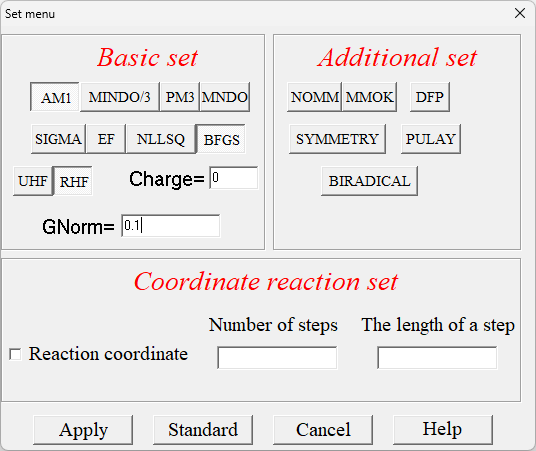
\includegraphics[width=0.5\textwidth]{image/set_menu1.png}
  \caption{Настройка параметров моделирования в WinMOPAC}
\end{figure}

Согласно синтаксису языка описания структур молекул в \textbf{WinMOPAC} геометрическое
описание начинаетс строго с $4$-ой строки, все строки до отдаются для описания параметров
моделирования и комментариев. Z-матрица задает начальное взаимное расположение двух атомов 
углерода и четырех атомов водорода в плоской симметричной конформации.

\begin{lstlisting}[style=mopac-block]
AM1 RHF BFGS CHARGE=0 GNORM=0.1 BONDS GEO-OK VECTORS DENSITY
lab 2 var 1
ethylene molecule C2H4
C   0.000000  0    0.000000  0    0.000000  0    0   0   0
C   1.340000  1    0.000000  0    0.000000  0    1   0   0
H   1.090000  1  121.000000  1    0.000000  0    1   2   0
H   1.090000  1  121.000000  1  180.000000  1    1   2   3
H   1.090000  1  121.000000  1    0.000000  1    2   1   3
H   1.090000  1  121.000000  1  180.000000  1    2   1   3
\end{lstlisting}

\textbf{RasWin} показывает визуализацию молекулы этилена в трехмерном пространстве, 
для кода выше она выглядит как на Рис. $\ref{fig:raswin}$.

\begin{figure}[H]
  \centering
  \begin{minipage}[t]{0.48\textwidth} 
    \centering
    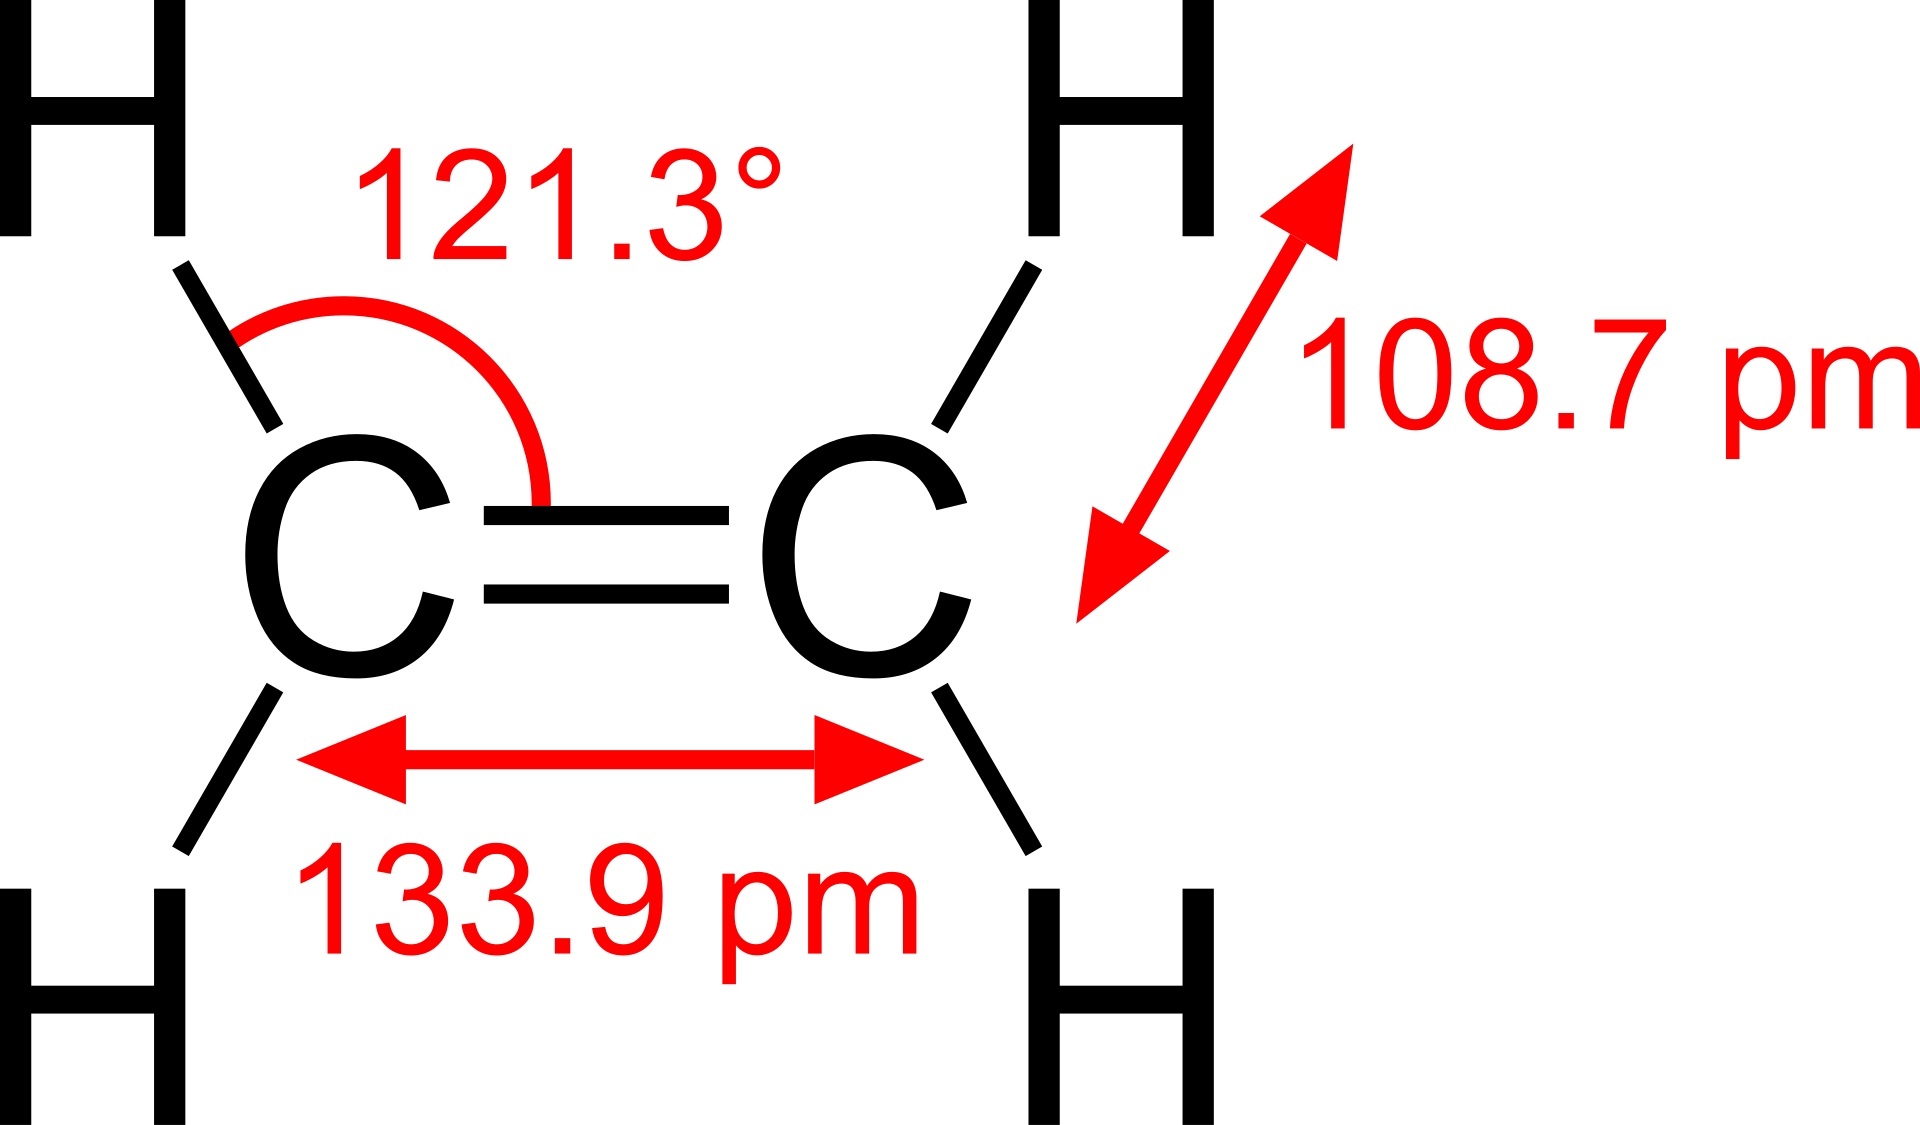
\includegraphics[width=\textwidth]{image/ethylene.png}
    \caption{Схематичное изображение молекулы этилена}
    \label{fig:ethylene}
  \end{minipage} \hfill
  \begin{minipage}[t]{0.48\textwidth}
    \centering
    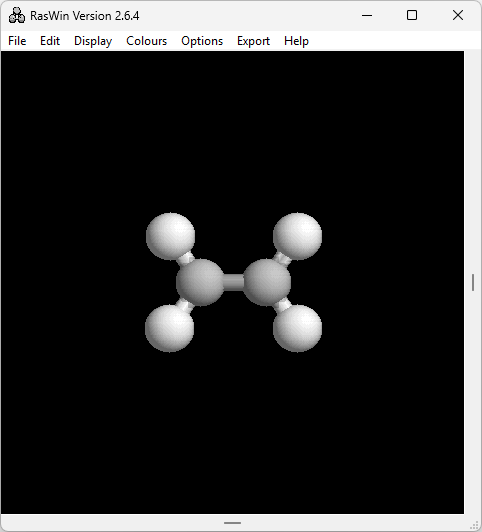
\includegraphics[width=\textwidth]{image/raswin.png}
    \caption{Визуализация молекулы этилена в \textbf{RasWin}}
    \label{fig:raswin}
  \end{minipage}
\end{figure}

Запуск вычислений оптимизации геометрии молекулы и энергического анализа производится
нажатием кнопки \textbf{Run WinMOPAC}. После завершения вычислений в окне
\textbf{Brief results} отображаются основные результаты расчета, а в окне
\textbf{Final matrix} — оптимизированные геометрические параметры молекулы этилена.

Результат выполнения в окне \textbf{Brief results} 
\begin{lstlisting}[style=mopac-block]
FINAL HEAT OF FORMATION =  15.40471 KCAL
TOTAL ENERGY            = -311.81626 EV
ELECTRONIC ENERGY       = -742.34198 EV
CORE-CORE REPULSION     =  430.52572 EV
IONIZATION POTENTIAL    =  10.17455
NO. OF FILLED LEVELS    =  6
MOLECULAR WEIGHT        =  28.054
COMPUTATION TIME        = 0 h 0 min 0 sec
\end{lstlisting}

Результат выполнения в окне \textbf{Final matrix} 
\begin{lstlisting}[style=mopac-block]
C     .0000000  0       .000000  0       .000000  0    0    0    0      -.0799
C    1.3347630  1       .000000  0       .000000  0    1    0    0      -.0799
H    1.0890712  1    123.199158  1       .000000  0    1    2    0       .0400
H    1.0890616  1    123.178171  1    179.993105  1    1    2    3       .0399
H    1.0891002  1    123.192970  1       .008086  1    2    1    3       .0400
H    1.0890907  1    123.172002  1   -179.998057  1    2    1    3       .0399
\end{lstlisting}

\begin{figure}[H]
  \centering
  \begin{minipage}[t]{0.48\textwidth} 
    \centering
    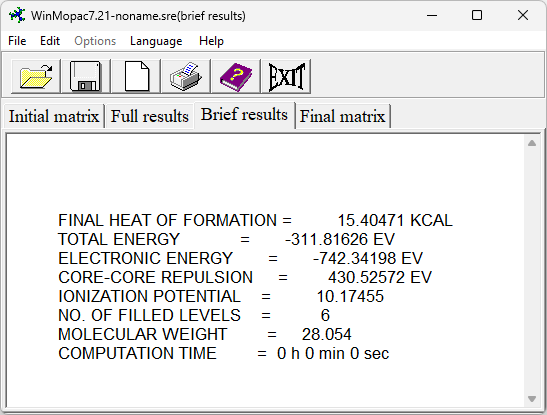
\includegraphics[width=\textwidth]{image/brief_results.png}
    \caption{Результаты расчета в окне Brief results}
  \end{minipage} \hfill
    \begin{minipage}[t]{0.48\textwidth} 
    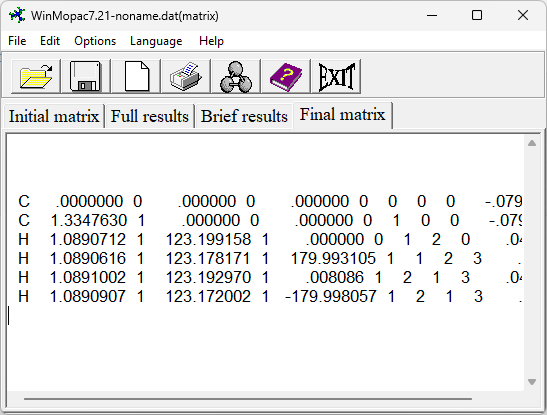
\includegraphics[width=\textwidth]{image/final_matrix.png}
    \caption{Результаты расчета в окне Final matrix}
  \end{minipage}
\end{figure}

\section{Вывод}

Вывод: кластер этилена был успешно смоделирован и оптимизирован. Расчёт показал 
устойчивость планарной компоновки (все диэдральные углы равны $0^\circ$ или $180^\circ$), 
а также симметричность молекулы (все углы при атомах водорода равны $123.2^\circ$).
Полученное значение молекулярной массы этилена равно $28.054$ г/моль, что соответствует 
данным из справочников и подтверждает корректность проведённого расчёта.

\end{document}